\documentclass[10pt]{article}
\usepackage[a4paper,margin=18mm]{geometry}
\usepackage{amsmath,amssymb,booktabs,array,enumitem}
\usepackage[T1]{fontenc}\usepackage{lmodern}
\usepackage{tikz}\usetikzlibrary{shapes.gates.logic.US,positioning,arrows.meta}
\usepackage[hidelinks]{hyperref}
\setlength{\parindent}{0pt}\setlength{\parskip}{4pt}\setlength{\emergencystretch}{2em}
\newcommand{\VDD}{V_{DD}}
\newcommand{\mos}[4]{\begin{scope}[shift={(#1,#2)}]
\draw(0,.23)--(0,-.23);\draw(0,.2)--(.25,.2)--(.25,.5);\draw(0,-.2)--(.25,-.2)--(.25,-.5);
\draw(-.16,.23)--(-.16,-.23);
\ifnum#4=1\draw(-.26,0)circle(.06);\draw(-.7,0)--(-.32,0);\else\draw(-.7,0)--(-.16,0);\fi
\node[anchor=east,font=\scriptsize]at(-.71,0){$#3$};\end{scope}}
\newcommand{\grd}[2]{\draw(#1,#2)--(#1,#2-.12);\draw(#1-.15,#2-.12)--(#1+.15,#2-.12);\draw(#1-.1,#2-.19)--(#1+.1,#2-.19);}
\newcommand{\sourcefigone}{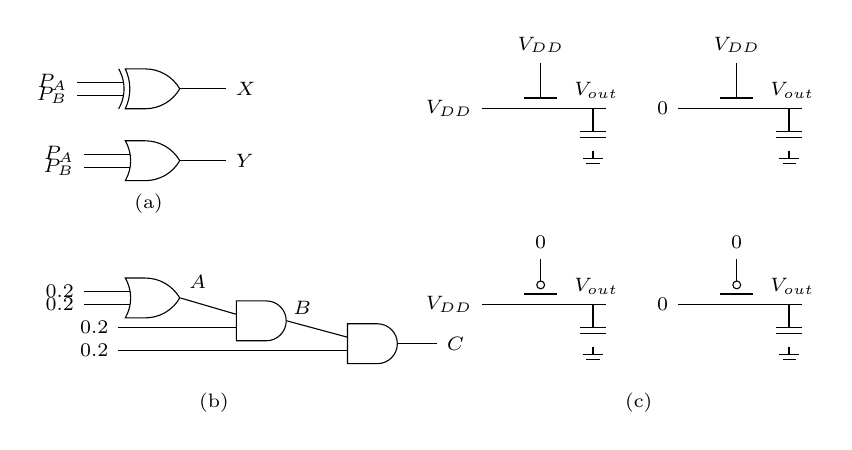
\begin{tikzpicture}[x=.83cm,y=.83cm,font=\scriptsize]
\node[xor gate US,draw,logic gate inputs=nn](x)at(1,4.3){};\node[or gate US,draw,logic gate inputs=nn](y)at(1,3.2){};
\foreach\g in{x,y}{\draw(\g.input 1)--++(-.7,0)node[left]{$P_A$};\draw(\g.input 2)--++(-.7,0)node[left]{$P_B$};}
\draw(x.output)--++(.7,0)node[right]{$X$};\draw(y.output)--++(.7,0)node[right]{$Y$};\node at(1,2.55){(a)};
\node[or gate US,draw,logic gate inputs=nn](a)at(1,1.1){};\node[and gate US,draw,logic gate inputs=nn](b)at(2.7,.75){};\node[and gate US,draw,logic gate inputs=nn](c)at(4.4,.4){};
\draw(a.input 1)--++(-.7,0)node[left]{0.2};\draw(a.input 2)--++(-.7,0)node[left]{0.2};\draw(a.output)--(b.input 1);\draw(b.input 2)--++(-1.8,0)node[left]{0.2};\draw(b.output)--(c.input 1);\draw(c.input 2)--++(-3.5,0)node[left]{0.2};
\node[above]at(1.75,1.1){$A$};\node[above]at(3.35,.7){$B$};\draw(c.output)--++(.6,0)node[right]{$C$};\node at(2,-.5){(b)};
\foreach\x/\yy/\gg/\in/\typ in{7/4/V_{DD}/V_{DD}/0,10/4/V_{DD}/0/0,7/1/0/V_{DD}/1,10/1/0/0/1}{
\draw(\x-.9,\yy)--(\x-.3,\yy) (\x+.3,\yy)--(\x+1,\yy);\draw(\x-.3,\yy)--(\x+.3,\yy);
\draw(\x-.25,\yy+.16)--(\x+.25,\yy+.16);\ifnum\typ=1\draw(\x,\yy+.3)circle(.06);\draw(\x,\yy+.36)--(\x,\yy+.7);\else\draw(\x,\yy+.16)--(\x,\yy+.7);\fi
\node[above]at(\x,\yy+.7){$\gg$};\node[left]at(\x-.9,\yy){$\in$};\node[above]at(\x+.85,\yy){$V_{out}$};\draw(\x+.8,\yy)--(\x+.8,\yy-.35);\draw(\x+.6,\yy-.35)--(\x+1,\yy-.35) (\x+.6,\yy-.45)--(\x+1,\yy-.45);\grd{\x+.8}{\yy-.65}}
\node at(8.5,-.5){(c)};\end{tikzpicture}}
\newcommand{\wirefig}{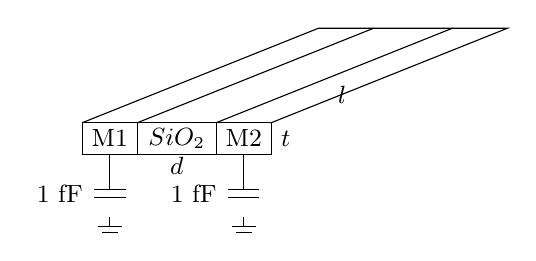
\begin{tikzpicture}[x=1cm,y=1cm,font=\small]
\draw(0,1)rectangle(.7,1.4);\draw(.7,1)rectangle(1.7,1.4);\draw(1.7,1)rectangle(2.4,1.4);
\draw(0,1.4)--(3,2.6)--(5.4,2.6)--(2.4,1.4);\draw(.7,1.4)--(3.7,2.6) (1.7,1.4)--(4.7,2.6);
\node at(.35,1.2){M1};\node at(1.2,1.2){$SiO_2$};\node at(2.05,1.2){M2};\node at(3.3,1.75){$l$};\node[right]at(2.4,1.2){$t$};\node at(1.2,.85){$d$};
\foreach\x in{.35,2.05}{\draw(\x,1)--(\x,.55);\draw(\x-.2,.55)--(\x+.2,.55) (\x-.2,.45)--(\x+.2,.45);\grd{\x}{.2}\node[left]at(\x-.22,.5){1 fF};}\end{tikzpicture}}
\newcommand{\chainsfig}{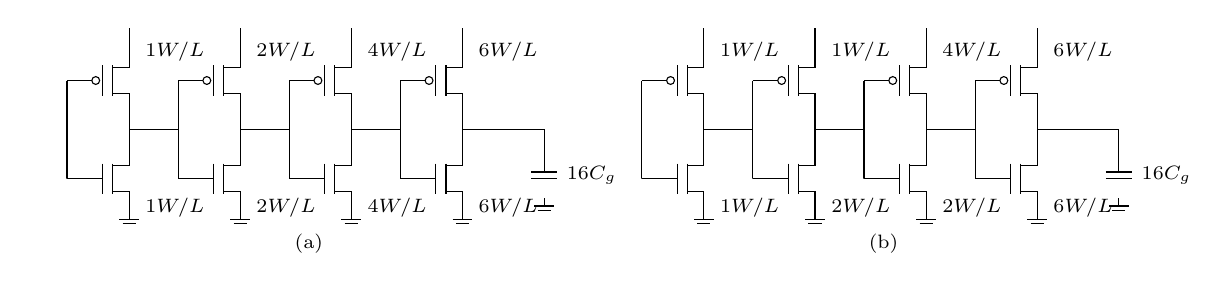
\begin{tikzpicture}[x=.83cm,y=.83cm,font=\scriptsize]
\begin{scope}[xshift=0cm]
\mos{0.0}{2.5}{\phantom{X}}{1}\mos{0.0}{1}{\phantom{X}}{0}
\draw(0.25,3)--(0.25,3.3);\draw(0.25,2)--(0.25,1.5);\grd{0.25}{.5}
\draw(-0.7,2.5)--(-0.7,1)--(-0.7,1.75);
\node[above right]at(0.35,2.65){$1W/L$};\node[below right]at(0.35,.85){$1W/L$};
\draw(0.25,1.75)--(1.0,1.75);
\mos{1.7}{2.5}{\phantom{X}}{1}\mos{1.7}{1}{\phantom{X}}{0}
\draw(1.95,3)--(1.95,3.3);\draw(1.95,2)--(1.95,1.5);\grd{1.95}{.5}
\draw(1.0,2.5)--(1.0,1)--(1.0,1.75);
\node[above right]at(2.05,2.65){$2W/L$};\node[below right]at(2.05,.85){$2W/L$};
\draw(1.95,1.75)--(2.7,1.75);
\mos{3.4}{2.5}{\phantom{X}}{1}\mos{3.4}{1}{\phantom{X}}{0}
\draw(3.65,3)--(3.65,3.3);\draw(3.65,2)--(3.65,1.5);\grd{3.65}{.5}
\draw(2.7,2.5)--(2.7,1)--(2.7,1.75);
\node[above right]at(3.75,2.65){$4W/L$};\node[below right]at(3.75,.85){$4W/L$};
\draw(3.65,1.75)--(4.4,1.75);
\mos{5.1}{2.5}{\phantom{X}}{1}\mos{5.1}{1}{\phantom{X}}{0}
\draw(5.35,3)--(5.35,3.3);\draw(5.35,2)--(5.35,1.5);\grd{5.35}{.5}
\draw(4.3999999999999995,2.5)--(4.3999999999999995,1)--(4.3999999999999995,1.75);
\node[above right]at(5.449999999999999,2.65){$6W/L$};\node[below right]at(5.449999999999999,.85){$6W/L$};
\draw(5.35,1.75)--(6.6,1.75)--(6.6,1.1);\draw(6.4,1.1)--(6.8,1.1) (6.4,1)--(6.8,1);\grd{6.6}{.7}\node[right]at(6.8,1.05){$16C_g$};
\node at(3,0){(a)};
\end{scope}
\begin{scope}[xshift=7.3cm]
\mos{0.0}{2.5}{\phantom{X}}{1}\mos{0.0}{1}{\phantom{X}}{0}
\draw(0.25,3)--(0.25,3.3);\draw(0.25,2)--(0.25,1.5);\grd{0.25}{.5}
\draw(-0.7,2.5)--(-0.7,1)--(-0.7,1.75);
\node[above right]at(0.35,2.65){$1W/L$};\node[below right]at(0.35,.85){$1W/L$};
\draw(0.25,1.75)--(1.0,1.75);
\mos{1.7}{2.5}{\phantom{X}}{1}\mos{1.7}{1}{\phantom{X}}{0}
\draw(1.95,3)--(1.95,3.3);\draw(1.95,2)--(1.95,1.5);\grd{1.95}{.5}
\draw(1.0,2.5)--(1.0,1)--(1.0,1.75);
\node[above right]at(2.05,2.65){$1W/L$};\node[below right]at(2.05,.85){$2W/L$};
\draw(1.95,1.75)--(2.7,1.75);
\mos{3.4}{2.5}{\phantom{X}}{1}\mos{3.4}{1}{\phantom{X}}{0}
\draw(3.65,3)--(3.65,3.3);\draw(3.65,2)--(3.65,1.5);\grd{3.65}{.5}
\draw(2.7,2.5)--(2.7,1)--(2.7,1.75);
\node[above right]at(3.75,2.65){$4W/L$};\node[below right]at(3.75,.85){$2W/L$};
\draw(3.65,1.75)--(4.4,1.75);
\mos{5.1}{2.5}{\phantom{X}}{1}\mos{5.1}{1}{\phantom{X}}{0}
\draw(5.35,3)--(5.35,3.3);\draw(5.35,2)--(5.35,1.5);\grd{5.35}{.5}
\draw(4.3999999999999995,2.5)--(4.3999999999999995,1)--(4.3999999999999995,1.75);
\node[above right]at(5.449999999999999,2.65){$6W/L$};\node[below right]at(5.449999999999999,.85){$6W/L$};
\draw(5.35,1.75)--(6.6,1.75)--(6.6,1.1);\draw(6.4,1.1)--(6.8,1.1) (6.4,1)--(6.8,1);\grd{6.6}{.7}\node[right]at(6.8,1.05){$16C_g$};
\node at(3,0){(b)};
\end{scope}
\end{tikzpicture}}
\newcommand{\qsevenfig}{\begin{tikzpicture}[x=1cm,y=.85cm,font=\small]
\mos{2}{6}{A}{1}\draw(2.25,6.5)--(2.25,6.9)node[above]{$V_{DD}$};
\draw(2.25,5.5)--(.75,5.5)--(.75,4.5) (2.25,5.5)--(3.75,5.5)--(3.75,5);
\mos{.5}{4}{B}{1}\mos{3.5}{4.5}{C}{1}\mos{3.5}{3}{D}{1}\draw(3.75,4)--(3.75,3.5);
\draw(.75,3.5)--(.75,2.3)--(3.75,2.3)--(3.75,2.5);\draw(2.25,2.3)--(5.2,2.3)node[right]{$F$};
\draw(2.25,2.3)--(.25,2.3)--(.25,1.4);\mos{0}{.9}{A}{0}\draw(.25,.4)--(.25,-1.1);
\draw(2.25,2.3)--(2.25,2);\mos{2}{1.5}{B}{0}\draw(2.25,1)--(2.25,.7)--(1.5,.7)--(1.5,.4) (2.25,.7)--(3.25,.7)--(3.25,.4);
\mos{1.25}{-.1}{C}{0}\mos{3}{-.1}{D}{0}\draw(1.5,-.6)--(1.5,-1.1)--(.25,-1.1) (3.25,-.6)--(3.25,-1.1)--(1.5,-1.1);\grd{1.5}{-1.1}
\end{tikzpicture}}
\newcommand{\aoifig}{\begin{tikzpicture}[x=1cm,y=.8cm,font=\small]
\mos{0}{4}{a}{1}\mos{2}{4.7}{b}{1}\mos{2}{3.3}{c}{1}\draw(.25,4.5)--(.25,5.4)--(2.25,5.4)--(2.25,5.2);\node[above]at(1.25,5.4){$V_{DD}$};\draw(2.25,4.2)--(2.25,3.8);
\draw(.25,3.5)--(.25,2.6)--(2.25,2.6)--(2.25,2.8);\draw(1.25,2.6)--(3.5,2.6)node[right]{$f$};
\mos{1}{2}{a}{0}\draw(1.25,2.6)--(1.25,2.5);\draw(1.25,1.5)--(.25,1.5)--(.25,1.2) (1.25,1.5)--(2.25,1.5)--(2.25,1.2);
\mos{0}{.7}{b}{0}\mos{2}{.7}{c}{0}\draw(.25,.2)--(.25,-.2)--(2.25,-.2)--(2.25,.2);\grd{1.25}{-.2}\end{tikzpicture}}
\begin{document}
\begin{center}{\Large\bfseries 2007 Midterm -- Corrected Solutions}\\EE3032, National Central University, Li\end{center}
\textbf{Scope.} All seven questions from the complete Fall 2007 original. The original percentages total \textbf{110\%}. The supplied handwriting is a comparison source, not an answer key; unfinished answers are derived here. No process-specific simulation is asserted.

\textbf{1. Brief answers}
\begin{enumerate}[label=(\alph*),leftmargin=7mm]
\item $f=\overline{a(b+c)}$: NMOS $a$ in series with $(b\parallel c)$; PMOS $a$ in parallel with series $b,c$. The dual networks give exactly one conducting rail for every Boolean input. Bodies: nMOS to $V_{SS}$, pMOS to $V_{DD}$.
\begin{center}\aoifig\end{center}
\item Clean the wafer; apply and bake photoresist; align the mask and expose; develop; transfer the opened pattern by etching (or perform the appropriate implantation); strip the resist and clean. The student's ``coat--expose--etch'' omits development, the step that creates the resist openings.
\item Reduce effective output/wire capacitance; lower path resistance by appropriate device sizing; reduce logic depth or use suitable buffering. Each targets the critical delay. Higher supply can also improve speed within the process limits, with an energy cost; increasing every width need not help because it loads the previous stage.
\item Use frequent low-resistance well/substrate taps and properly biased guard rings; increase separation or use an isolation process such as SOI/deep-trench isolation.
\item From $P_{sw}=\alpha_{01}fC_LV_{DD}^{2}$, reduce supply, switched capacitance, and switching activity/required event frequency. Avoid unnecessary glitches; preserve the required throughput.
\item Design rules specify manufacturable widths, spacings, overlaps and enclosure, including tolerances for lithography and alignment. They connect the layout to reliable fabrication. Communication between designers is useful but is not their principal physical purpose.
\item Reverse source--body bias increases threshold magnitude by changing the depletion charge. For NMOS,
\[V_T=V_{T0}+\gamma\bigl(\sqrt{2\phi_F+V_{SB}}-\sqrt{2\phi_F}\bigr).\]
The effective source is the lower-potential channel terminal for NMOS; a pass-device source need not be the left terminal.
\item A $p^+$ substrate ring tied to $V_{SS}$ and an $n^+$ well ring tied to $V_{DD}$ collect injected carriers and reduce substrate/well voltage drops. This suppresses triggering of the parasitic regenerative pnp--npn path.
\item For $0\to V_{DD}$ at the output, the supply provides $C_LV_{DD}^2$; $\tfrac12C_LV_{DD}^2$ is stored and the other half dissipates in the charging path. Discharging dissipates the stored half. A full $0\to1\to0$ cycle consumes $C_LV_{DD}^2$ from the supply, plus any short-circuit/leakage contribution. One output fall does not independently draw another $C_LV_{DD}^2$.
\end{enumerate}
\newpage
\textbf{2. Pass-transistor multiplexer and TG XOR}

(a) Use a three-level binary tree of two-input NMOS pass multiplexers. Each mux has two physical nMOS switches: $D_0$ gated by $\bar S$ and $D_1$ gated by $S$. This is \textbf{14 nMOS}, plus three inverters (six MOS) if the complementary selects are generated locally. Each selected path has three conducting pass devices. An all-high data value is a weak high, approximately $V_{DD}-V_{Tn}$ with possible body effect; it is not three successive threshold drops when all gates are driven by a full-rail select. Add a restoring buffer if full-rail logic is required.
\begin{center}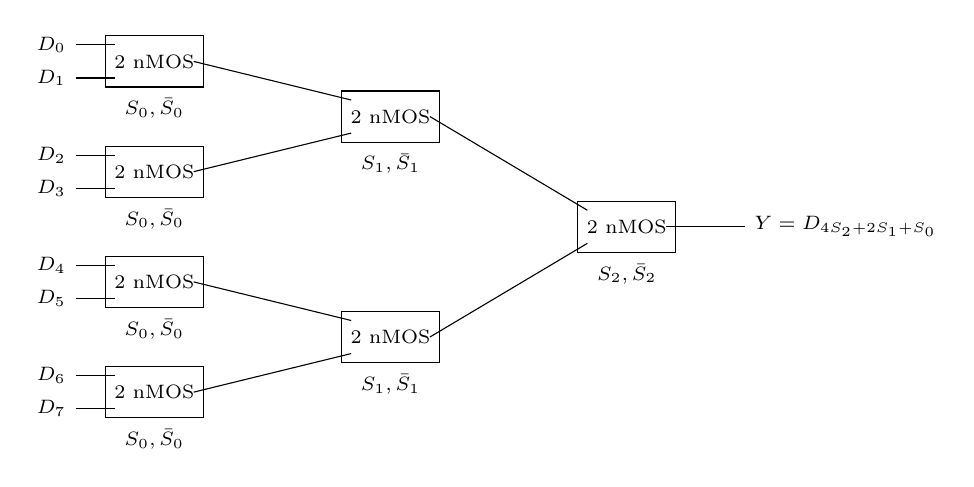
\begin{tikzpicture}[x=1cm,y=.7cm,font=\scriptsize]
\foreach\i in{0,...,3}{\node[draw,minimum width=1cm,minimum height=.65cm](m\i)at(1,{6-2*\i}){2 nMOS};\draw(0,{6.3-2*\i})--(.5,{6.3-2*\i})node[pos=0,left]{$D_{\the\numexpr2*\i\relax}$};\draw(0,{5.7-2*\i})--(.5,{5.7-2*\i})node[pos=0,left]{$D_{\the\numexpr2*\i+1\relax}$};\node[below]at(1,{5.5-2*\i}){$S_0,\bar S_0$};}
\foreach\i in{0,1}{\node[draw,minimum width=1cm,minimum height=.65cm](n\i)at(4,{5-4*\i}){2 nMOS};\draw(1.5,{6-4*\i})--(3.5,{5.3-4*\i});\draw(1.5,{4-4*\i})--(3.5,{4.7-4*\i});\node[below]at(4,{4.5-4*\i}){$S_1,\bar S_1$};}
\node[draw,minimum width=1cm,minimum height=.65cm]at(7,3){2 nMOS};\draw(4.5,5)--(6.5,3.3);\draw(4.5,1)--(6.5,2.7);\draw(7.5,3)--(8.5,3)node[right]{$Y=D_{4S_2+2S_1+S_0}$};\node[below]at(7,2.5){$S_2,\bar S_2$};
\end{tikzpicture}\end{center}
Each labelled block contains the two switches defined above; the gate terminal labels specify the complete transistor implementation.

(b) $Y=A\oplus B=\bar A B+A\bar B$. A two-branch TG mux passes $B$ when $A=0$ and $\bar B$ when $A=1$.
\begin{center}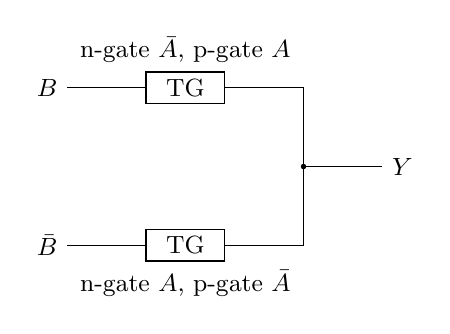
\begin{tikzpicture}[font=\small]
\draw(0,1)--(1,1);\node[left]at(0,1){$B$};\draw(1,.8)rectangle(2,1.2);\node at(1.5,1){TG};\node[above]at(1.5,1.2){n-gate $\bar A$, p-gate $A$};
\draw(0,-1)--(1,-1);\node[left]at(0,-1){$\bar B$};\draw(1,-1.2)rectangle(2,-.8);\node at(1.5,-1){TG};\node[below]at(1.5,-1.2){n-gate $A$, p-gate $\bar A$};
\draw(2,1)--(3,1)--(3,-1)--(2,-1);\draw(3,0)--(4,0)node[right]{$Y$};\fill(3,0)circle(.035);
\end{tikzpicture}\end{center}
Two TGs use four MOS; local $A/B$ complement generation adds four MOS, total eight. The PDF student's cascaded pass array does not specify the required complementary pMOS/nMOS TG pairs. The photographed student's static-CMOS XOR uses a different implementation from the requested TG circuit. The two-TG mux above answers the specified technique directly.
\newpage
\textbf{3. Signal probability, transition activity, and pass levels}

\textbf{Distinguish occupancy from transition probability.} Let $p=P(Q=1)$. The identity $P(Q_t=0,Q_{t+1}=1)=p(1-p)$ requires successive samples to be independent with the same marginal distribution. The printed assumption for Q3(a) only states independence of $A$ and $B$, not independence over time. A constant random input word and an independently redrawn word can have the same marginal $p$ but different switching. Thus the requested activities are not unique without a temporal model.

(a) Same-sample independence gives
\[p_X=P_A(1-P_B)+(1-P_A)P_B,\qquad p_Y=P_A+P_B-P_AP_B.\]
Under the additional standard independent-sample model, $\alpha_X=p_X(1-p_X)$ and $\alpha_Y=p_Y(1-p_Y)$. With a general stationary sequence, write $\alpha_Q=p_Q-P(Q_t=1,Q_{t+1}=1)$.

(b) With \emph{independent input bits and independent successive samples}, the cascaded logic is $A=U+V$, $B=AW$, $C=BT$ and the numerical values are
\begin{center}\begin{tabular}{ccc}\toprule Node&$p_1$&$P_{0\to1}$ under the stated extra model\\\midrule
$A$&$1-.8^2=.36$&$.36(.64)=.2304$\\
$B$&$.36(.2)=.072$&$.072(.928)=.066816$\\
$C$&$.072(.2)=.0144$&$.0144(.9856)=.01419264$\\\bottomrule\end{tabular}\end{center}
The original gives only 0.2 marginal occupancies in (b); correlation between bits or samples invalidates these products. These are model-qualified activities, not results forced by the original marginals. The photographed student interchanges the XOR/OR labels and uses uniform-input truth-table proportions for (a), which do not apply to arbitrary $P_A,P_B$. In (b), multiplying the previous node's transition activity by .2 is not the same as recomputing activity from the new node's occupancy. The PDF set leaves this question unfinished.

(c) At the ideal constant-threshold level, in the order upper left, upper right, lower left, lower right:
\begin{center}\begin{tabular}{p{25mm}p{44mm}p{59mm}}\toprule Device/data&Output&Effective source / drain during transfer\\\midrule
nMOS / $V_{DD}$&$V_{DD}-V_{Tn}$&output lower: source; data higher: drain\\
nMOS / 0&0&data lower: source; output initially higher: drain\\
pMOS / $V_{DD}$&$V_{DD}$&data higher: source; output initially lower: drain\\
pMOS / 0&$|V_{Tp}|$&output initially higher: source; data lower: drain\\\bottomrule\end{tabular}\end{center}
Weak-level limits assume the capacitor starts on the side that can move toward the quoted level. A floating node initially below $|V_{Tp}|$ is not actively charged to that level by an OFF pMOS connected to zero. When potentials equal, source/drain naming is interchangeable. Body effect makes the threshold limits implicit; for an nMOS passing high, solve $V_{out}=V_{DD}-V_{Tn}(V_{out})$. The student's voltage limits are the conventional ideal limits, but fixed left/right source labels omit their dependence on voltage and initial state.

\textbf{4. Capacitive crosstalk}
\[C_c=\epsilon\frac{tl}{d}=5\times10^{-14}\frac{(10^{-4})(10^{-2})}{10^{-4}}\,\mathrm F=5\times10^{-16}\,\mathrm F=.5\,\mathrm{fF}.\]
For a floating victim initially at zero, conserved victim-node charge gives
\[\Delta V_{M2}=\frac{C_c}{C_c+C_g}\Delta V_{M1}=\frac{.5}{.5+1}(1.8)=\boxed{.6\,\mathrm V}.\]
Here $C_g=1\,\mathrm{fF}$ is the victim's ground capacitance. The aggressor's 1 fF does not enter this divider when its voltage is driven as specified. The student's .6 V is independently confirmed.
\newpage
\textbf{5. Short-circuit power: account for both polarities and device strengths}

All widths in Figure 3 are read literally. Equal p/n widths are \emph{not} balanced here: $\mu_n=2\mu_p$, so $R_n=R/w_n$ and $R_p=2R/w_p$. With no drain/wire capacitance, the following transition-time estimates are in $RC_g$ units:
\begin{center}\begin{tabular}{ccccccc}\toprule Chain&Stage&$w_p$&$w_n$&$C_{out}/C_g$&$t_r/RC_g$&$t_f/RC_g$\\\midrule
(a)&1&1&1&4&8&4\\ &(2)&2&2&8&8&4\\ &(3)&4&4&12&6&3\\ &(4)&6&6&16&$16/3$&$8/3$\\\midrule
(b)&1&1&1&3&6&3\\ &(2)&1&2&6&12&3\\ &(3)&4&2&12&6&6\\ &(4)&6&6&16&$16/3$&$8/3$\\\bottomrule\end{tabular}\end{center}
\textbf{Classroom conclusion: (a) has slightly lower short-circuit power under a common square-law overlap approximation.} It is incorrect to identify short-circuit power just with the switched output capacitance. Chain (b) has less total switched capacitance ($37C_g$ versus $40C_g$), which answers a different power component.

Because the pairs are unbalanced, the equal-$\beta$ formula must be generalized. Let $\beta_n=\beta_0w_n$, $\beta_p=\beta_0w_p/2$, $\Delta=V_{DD}-V_{Tn}-|V_{Tp}|>0$, and
\[b(\beta_n,\beta_p)=\frac{\beta_n\beta_p}{(\sqrt{\beta_n}+\sqrt{\beta_p})^2}.\]
For a linear input ramp, the approximate overlap current is $\tfrac12\min\{\beta_n u^2,\beta_p(\Delta-u)^2\}$. Integrating the two branches on either side of $u=\sqrt{\beta_p}\Delta/(\sqrt{\beta_n}+\sqrt{\beta_p})$ yields
\[P_{sc}\simeq\frac{f\Delta^3}{6}\sum_i b_i(t_{r,in,i}+t_{f,in,i}).\]
This reduces to $\beta\tau\Delta^3f/12$ for a balanced inverter with $t_{r,in}=t_{f,in}=\tau$. First-stage contributions cancel because both chains have the same first pair and external input. Let $q=3-2\sqrt2$, so $b_{a,i}/\beta_0=q[1,2,4,6]$ and $b_{b,i}/\beta_0=[q,2/9,1/2,6q]$. The last three stages give
\begin{align*}
S_a/(\beta_0RC_g)&=2q(8+4)+4q(8+4)+6q(6+3)=126q,\\
S_b/(\beta_0RC_g)&=(2/9)(6+3)+(1/2)(12+3)+6q(6+6)=19/2+72q,\\
(S_b-S_a)/(\beta_0RC_g)&=19/2-54q\approx .235065>0.
\end{align*}
The advantage is small in this declared model. The photographed student chooses (b) by adding unweighted rise/fall times; that omits the different overlap-current strengths of the stages. The PDF set leaves Q5 blank. \textbf{A universal physical ordering is not determined by $R,C_g,\mu_n/\mu_p$ alone}: the exam omits thresholds, waveform shape, frequency and a finite-load current model. Loading suppresses actual overlap current and changes output slews. The result above is an explicit analytical classroom estimate; it is not a claimed SPICE measurement. If $\Delta\le0$, this ideal overlap model predicts zero for both, rather than a strict ordering.
\newpage
\textbf{6. Quadratic wire delay and repeater position}
The intended uniform distributed-RC wire model is $t_w=k l^2$; fixed external loads/driver delay are outside this exercise. Thus
\[t_w(100\,\mu\mathrm m)=.13(100/50)^2=\boxed{.52\,\mathrm{ps}}.\]
If an ideal isolating inverter is placed at $x$ along the 100-$\mu$m line,
\[t(x)=k[x^2+(100-x)^2]+.2,\quad k=.13/50^2\;\mathrm{ps}/\mu\mathrm m^2.\]
$t'(x)=k(4x-200)=0$ and $t''(x)=4k>0$ give $x=50\,\mu\mathrm m$. The minimum is $\boxed{.13+.2+.13=.46\,\mathrm{ps}}$. This independently confirms the student's result and retains the printed ps units. The output polarity is inverted by the inserted repeater.

\textbf{7. Width sizing with every channel length fixed}
The pull-down is $A\parallel[B(C\parallel D)]$; the dual pull-up is $A[B\parallel(CD)]$. Let $R_{n0},R_{p0}$ be the reference inverter's n/p resistance. Resistance scales inversely with width separately within each device type.
\begin{center}\begin{tabular}{cccc}\toprule Gate&$W_n$&$W_p$&$L_n=L_p$\\\midrule
$A$&$4\lambda$&$30\lambda$&$2\lambda$\\
$B$&$8\lambda$&$15\lambda$&$2\lambda$\\
$C$&$8\lambda$&$30\lambda$&$2\lambda$\\
$D$&$8\lambda$&$30\lambda$&$2\lambda$\\\bottomrule\end{tabular}\end{center}
The three minimal nMOS discharge paths have resistance $R_{n0}$, $(1/2+1/2)R_{n0}$, and $(1/2+1/2)R_{n0}$. The pMOS charge paths are
\[A,B:\;(1/3+2/3)R_{p0}=R_{p0},\qquad A,C,D:\;(1/3+1/3+1/3)R_{p0}=R_{p0}.\]
If multiple parallel branches conduct, resistance is smaller, so these establish the worst case. This is one valid equal-path sizing, not a unique optimum. The source does not ask minimum area.
\begin{center}\qsevenfig\end{center}
Associate each drawn gate with the width table above. The PDF student changes channel lengths to $4\lambda$ and $6\lambda$, contrary to the explicit fixed-$2\lambda$ requirement. The photographed set keeps the lengths fixed and correctly uses $30\lambda$ for pMOS A/C/D, but uses only $10\lambda$ for pMOS B. Its A--B charge path is then $(1/3+1)R_{p0}=4R_{p0}/3$, slower than the reference. Raising B to $15\lambda$ repairs this path while keeping all lengths fixed. The photographed nMOS widths are independently confirmed.

\textbf{Verification.} Saved switch-graph tables exhaust all 8 AOI21 inputs, all 2,048 mux data/select combinations, all four XOR inputs and all 16 sized-gate inputs. Exact rational path checks and independent weighted probability enumeration accompany the power/crosstalk/wire calculations. These are ideal-model checks, not fabricated process results.

\textbf{References.} The independent calculations use the original's assumptions. Physical mechanisms and standard delay/power vocabulary are cross-checked against the instructor's \href{https://www.ee.ncu.edu.tw/jfli/public_html/VLSI/lecture/ch04.pdf}{Electrical Characteristics of CMOS} and \href{https://www.ee.ncu.edu.tw/jfli/public_html/VLSI/lecture/ch05.pdf}{Circuit Design}, and \href{https://www.ti.com/lit/an/scla020a/scla020a.pdf}{TI's latchup discussion}. No source is an official answer key for this exam.
\end{document}
